\chapter{Solución propuesta}
\label{chap-solution}

En esta Sección se describen las técnicas aplicadas para lograr el seguimiento
de los jugadores. Primero se detallan algoritmos utilizados para ignorar los
elementos del fondo de la imagen en la Sección
\ref{sec:background-elimination}, y luego como fue utilizado el algoritmo
contornos activos (ver \cite{fast-level-set}) y las modificaciones que se le
hicieron en la Sección \ref{sec:ac-extension}. Finalmente, en la Sección
\ref{sec:alg-final} se detalla la integración final entre las distintas
técnicas, que es analizada en el siguiente Capítulo.

\section{Eliminación de fondo}
%% TODO: Ojo, a partir de acá hablamos en pasado. Deberíamos ser consistentes,
%% por como arrancamos en el resuemen, la intro y por lo que dice la mina
%% deberiamos usar el presente o eso de "se plantea, se define, etc..."

\label{sec:background-elimination}
% TODO: REEMPLAZAR PLANTEA por mejor palabra
Se planteó que el análisis por contornos activos se beneficia de un análisis
previo que detecte e informe a la actualización del contorno sobre sectores de
los cuadros del video que sin duda no corresponden a las siluetas de los
objetos de interés para el seguimiento.

Con ese fin, se analizan distintos métodos para extraer información adicional
de la imágen y detectar con el objetivo de ignorar sectores de la imágen que
no correspondan a jugadores con total certeza.

\subsection{Tribuna y publicidades}

La técnica más simple de eliminación de sectores es una técnica de
\textit{crop} que muestra como negro todo sector de la imágen ajeno a un
cuadrilátero que bordea la cancha.

\begin{figure}[H]
  \centering
    \begin{minipage}[t]{.45\textwidth}
      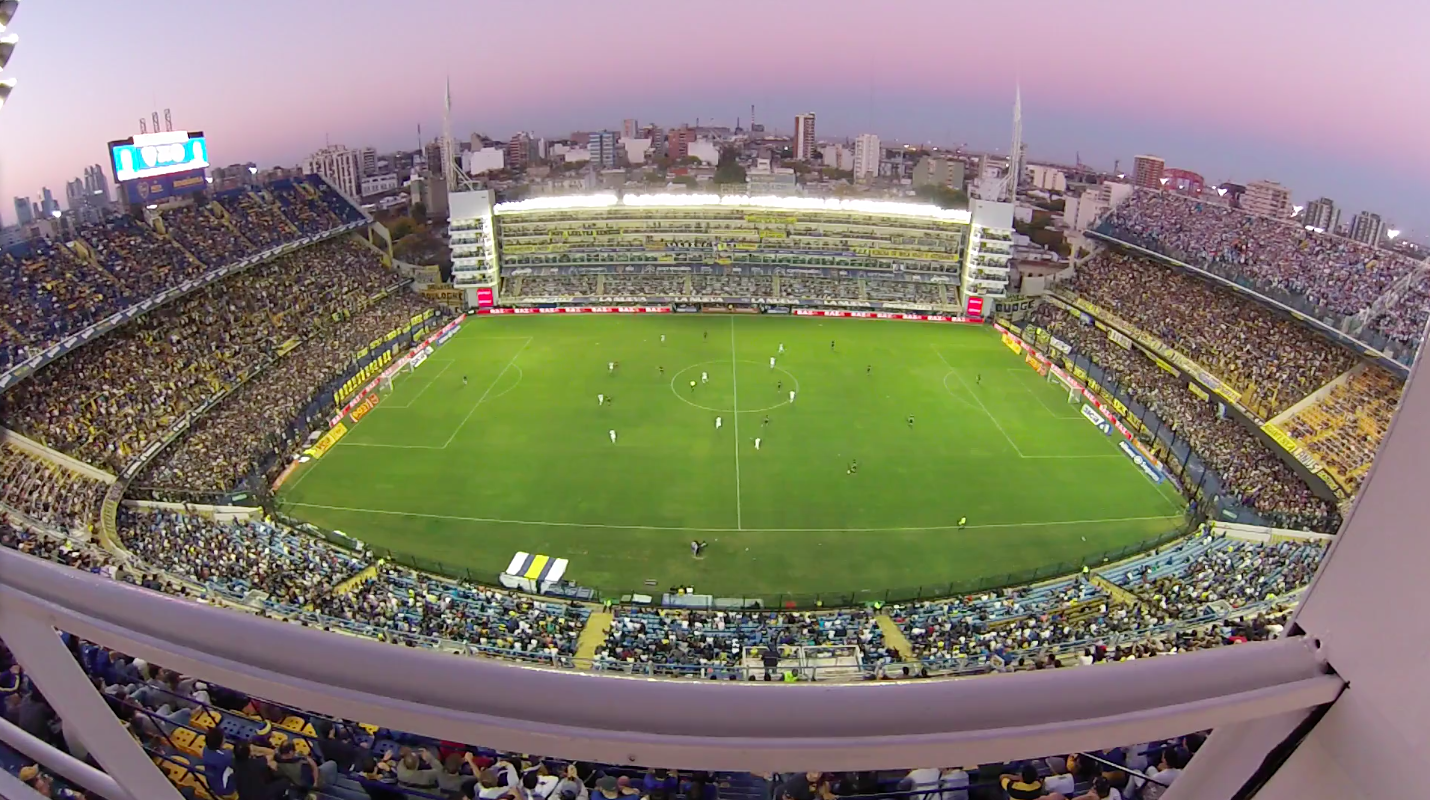
\includegraphics[width=\linewidth]{./images/Crop_Antes.png}
      \caption{Un cuadro del video de un partido entre Boca e Independiente.
      \label{fig:crop-antes}}
    \end{minipage}
    \begin{minipage}[t]{.45\textwidth}
      \centering
      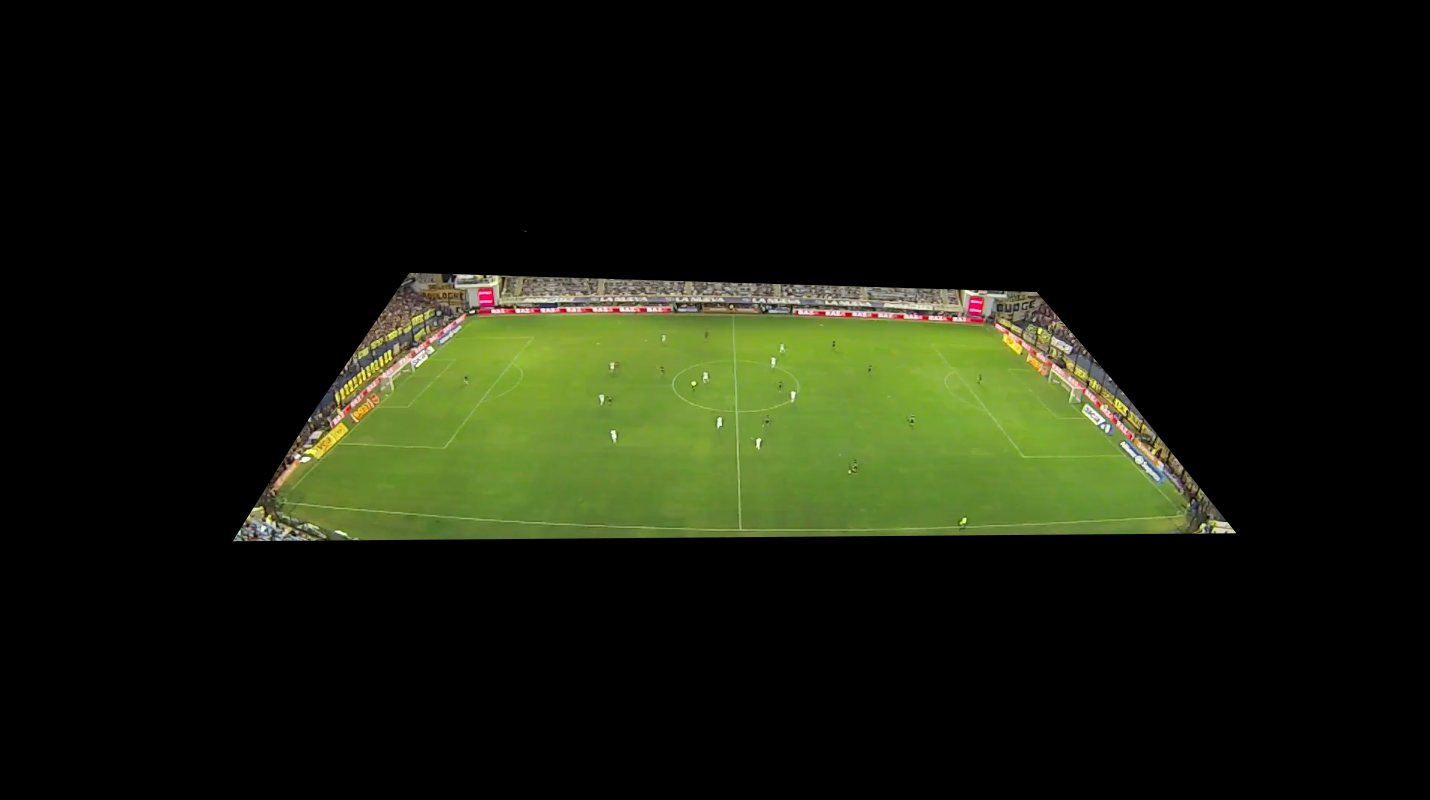
\includegraphics[width=\linewidth]{./images/Crop_Despues.png}
      \caption{El mismo cuadro, luego de aplicarle la operación \textit{Crop}.
      \label{fig:crop-despues}}
    \end{minipage}
\end{figure}

\subsection{Energía}

Se implementó el método de eliminación de fondo descripto en
\cite{papers-tanos}, para eliminación de sectores que corresponden al
verde del pasto de la cancha o líneas pintadas sobre el mismo basado
en una medición de la variación del color de cada píxel.

% TODO: Imágenes de cómo funciona

\subsection{Eliminación de lineas}

Basado en la detección de líneas de Hough, se desarrolló un método similar que
detecta los tramos pintados de blanco en el césped de la cancha. El mismo
funciona aplicando un detector de bordes (se probaron resultados utilizando
tanto el método de Roberts como el de Canny), umbralizando el resultado, y
haciendo un análisis morfológico de las componentes conexas obtenidas luego de
la umbralización.

Respecto a la detección de líneas de Hough, este método tiene la ventaja de que
% TODO

\subsection{Eliminación del pasto}
  * Eliminación de colores de cancha por histograma de colores

\section{Contornos activos}
\label{sec:ac-extension}

- Características

  * Colores del jugador
  * Aprendizaje
  * Múltiples características
  * Selección de máximos en histograma con bfs

- Descriptores

\section{Algoritmo final}
\label{sec:alg-final}
% Que onda esta seccion? Me parece medio tirada de los pelos la idea

- Eliminación de lineas por detector de borde + umbral + morfología
- Múltiples características
- Descriptores
- Imágenes de cómo resolvemos algunos casos extremos

- Opcional para equipos difíciles de detectar: seguimiento por complemento
  - eliminación de colores de cancha por histograma + ronda de contornos

- Que lastima que no tuvimos trackeo de pelota porque hubiese dado mejores datos
